%---------------------------------------------------------------------
\section{Observed Results}
\label{results}

This section presents the matrix element results obtained using the
$\sim$1~fb$^{-1}$ data set.

Figures~\ref{e21_2j} and~\ref{e21_3j} show the $tb$ and $tqb$
discriminants for the combined $e$,$\mu$ / 1,2 tags events for two-jet
and three-jet events where the data distributions may be compared to
the background model.  The SM prediction for single top quark
production has been added to the background sum in the plots. The
individual channel plots for the 1D discriminants are shown in
Appendix~\ref{Channel}.

\vspace{-0.05in}
\begin{figure}[!h!tbp]
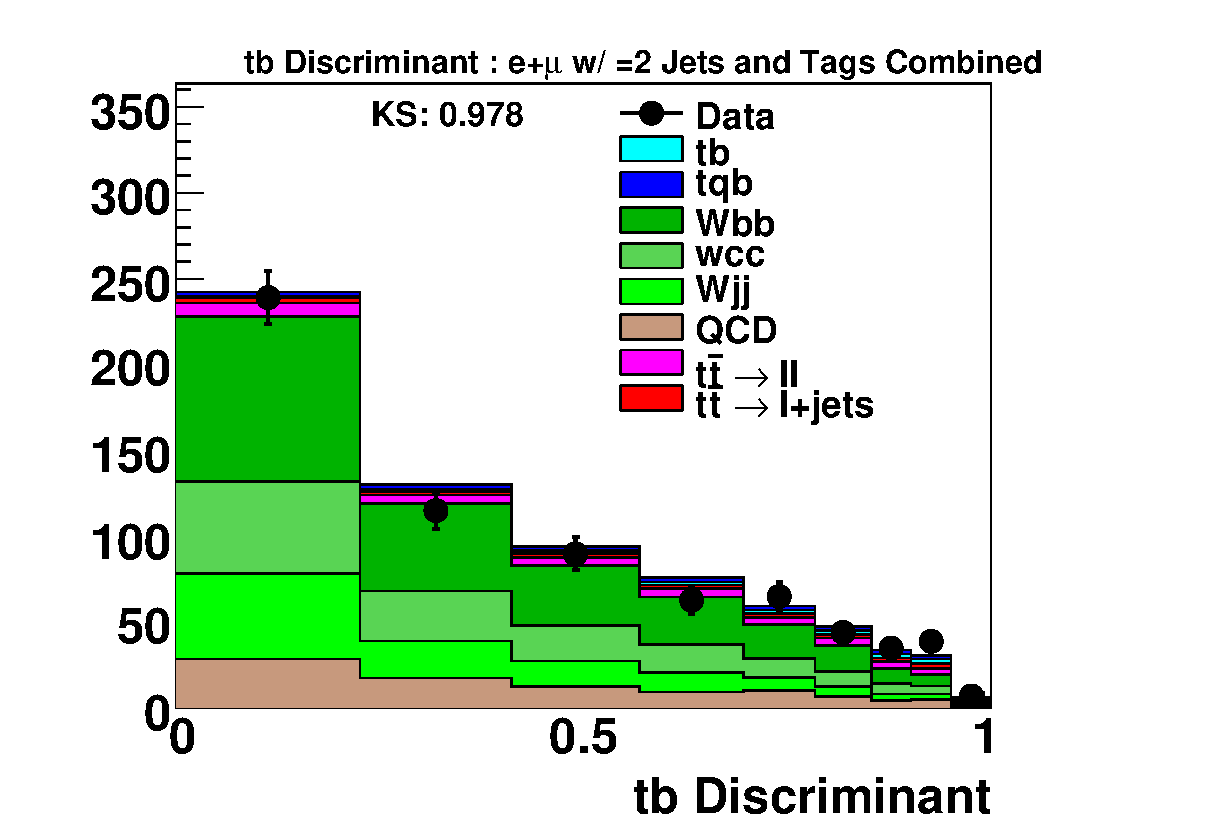
\includegraphics[width=0.36\textwidth]
{figures/output/2jet/All_tb_Discriminant.eps}
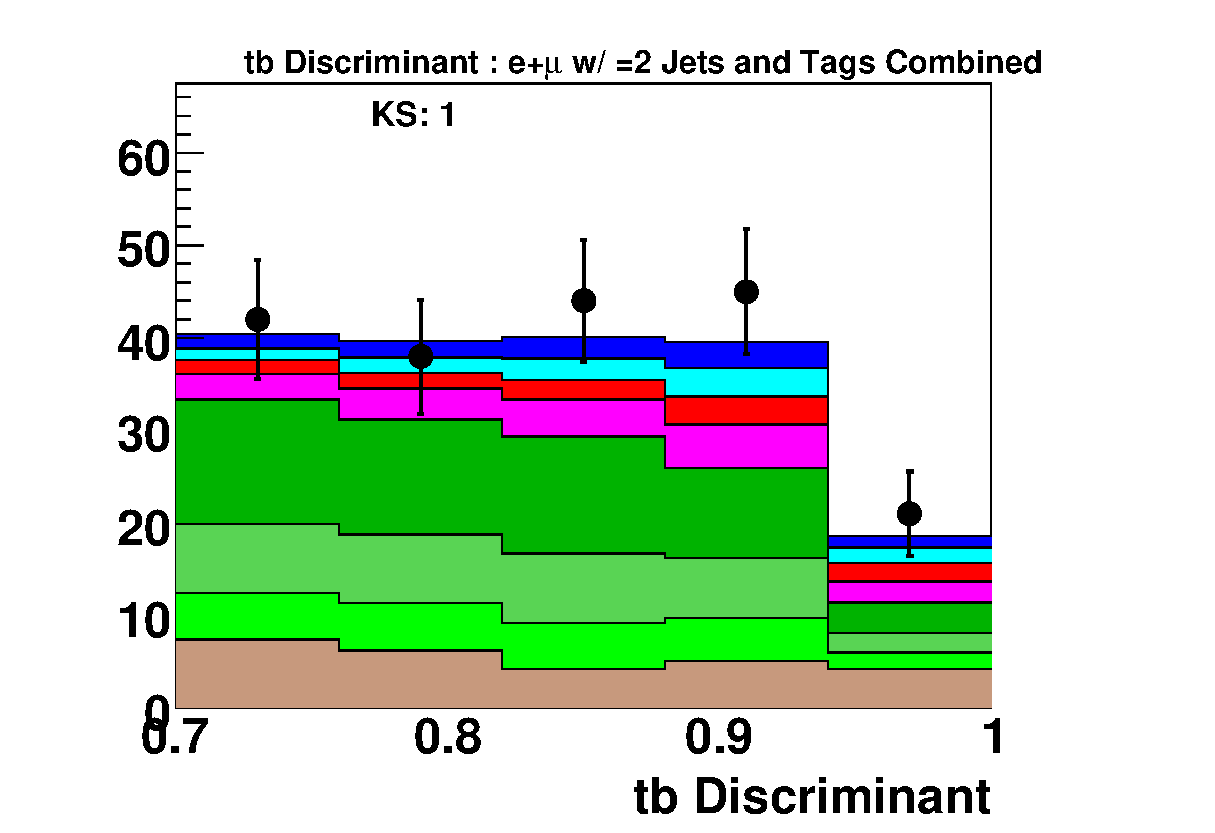
\includegraphics[width=0.36\textwidth]
{figures/output/2jet/All_tb_Discriminant_Zoom.eps}
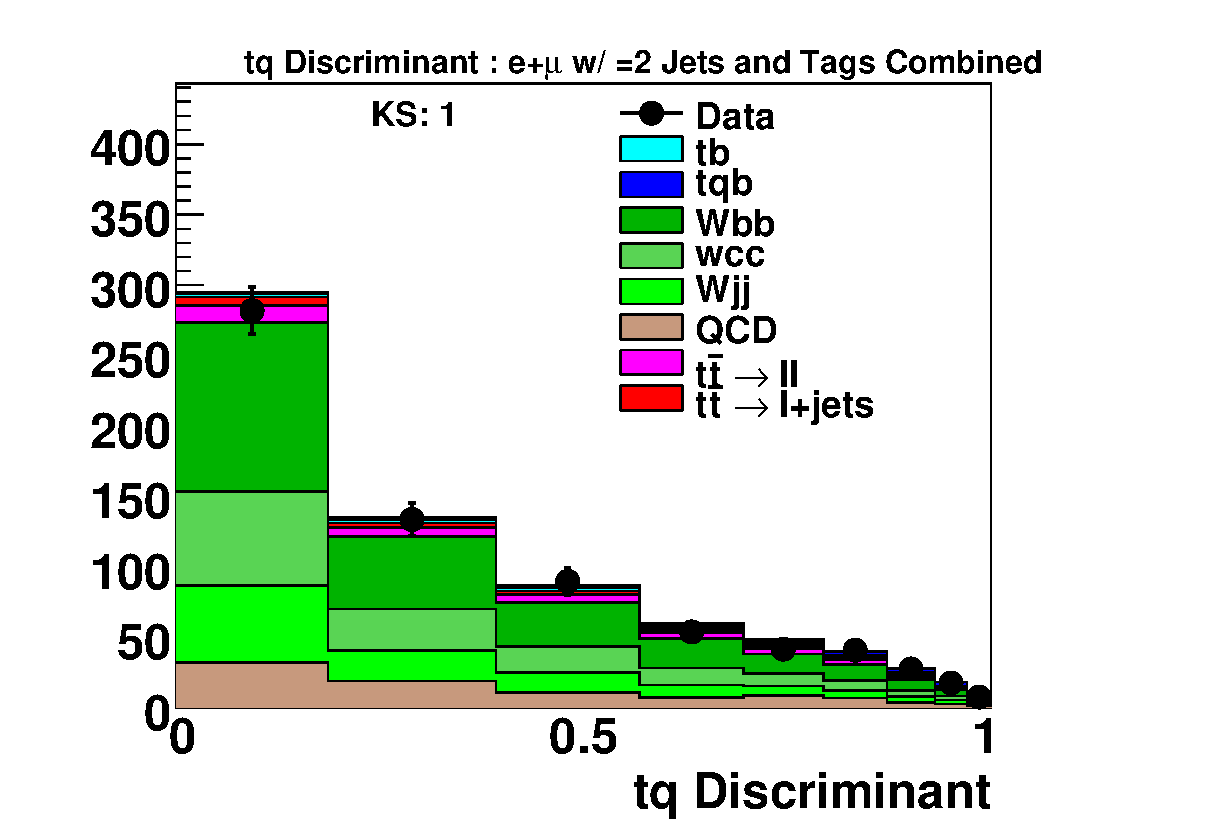
\includegraphics[width=0.36\textwidth]
{figures/output/2jet/All_tq_Discriminant.eps}
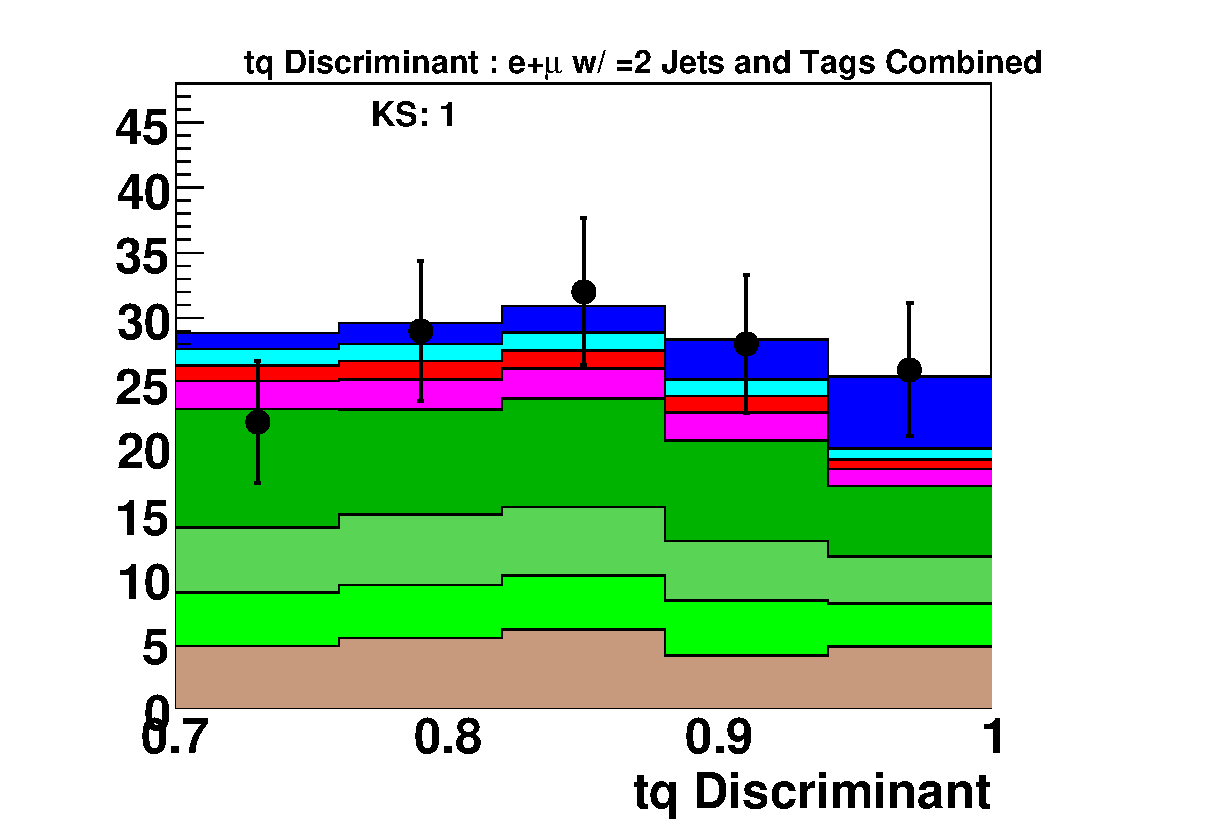
\includegraphics[width=0.36\textwidth]
{figures/output/2jet/All_tq_Discriminant_Zoom.eps}
\vspace{-0.1in}
\caption{Discriminant plots for the e+$\mu$ channel with two jets and
$\geq$~1 $b$~tag. Upper row: $tb$ discriminant; lower row: $tq$
discriminant. Left column: full output range; right column: close-up
of the high end of the distributions.}
\label{e21_2j}
\end{figure}

\vspace{-0.05in}
\begin{figure}[!h!tbp]
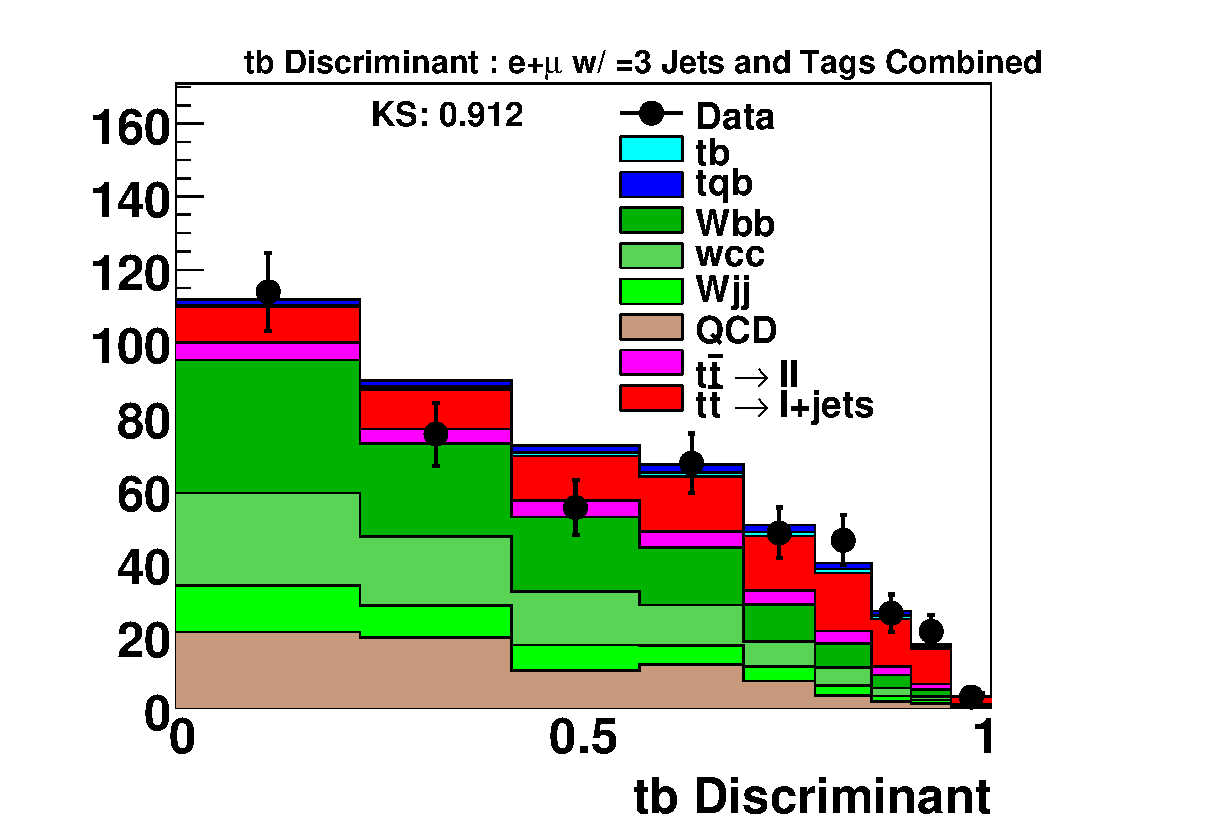
\includegraphics[width=0.36\textwidth]
{figures/output/3jet/All_tb_Discriminant.eps}
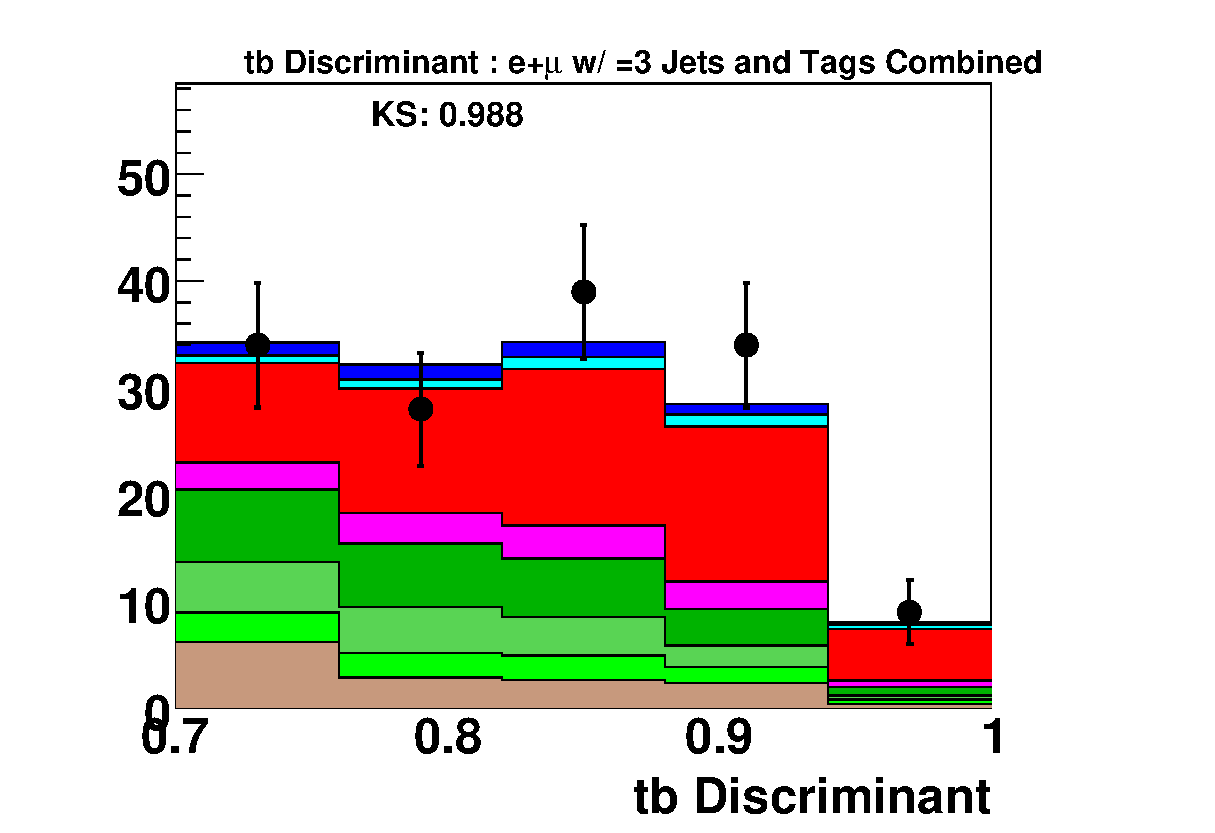
\includegraphics[width=0.36\textwidth]
{figures/output/3jet/All_tb_Discriminant_Zoom.eps}
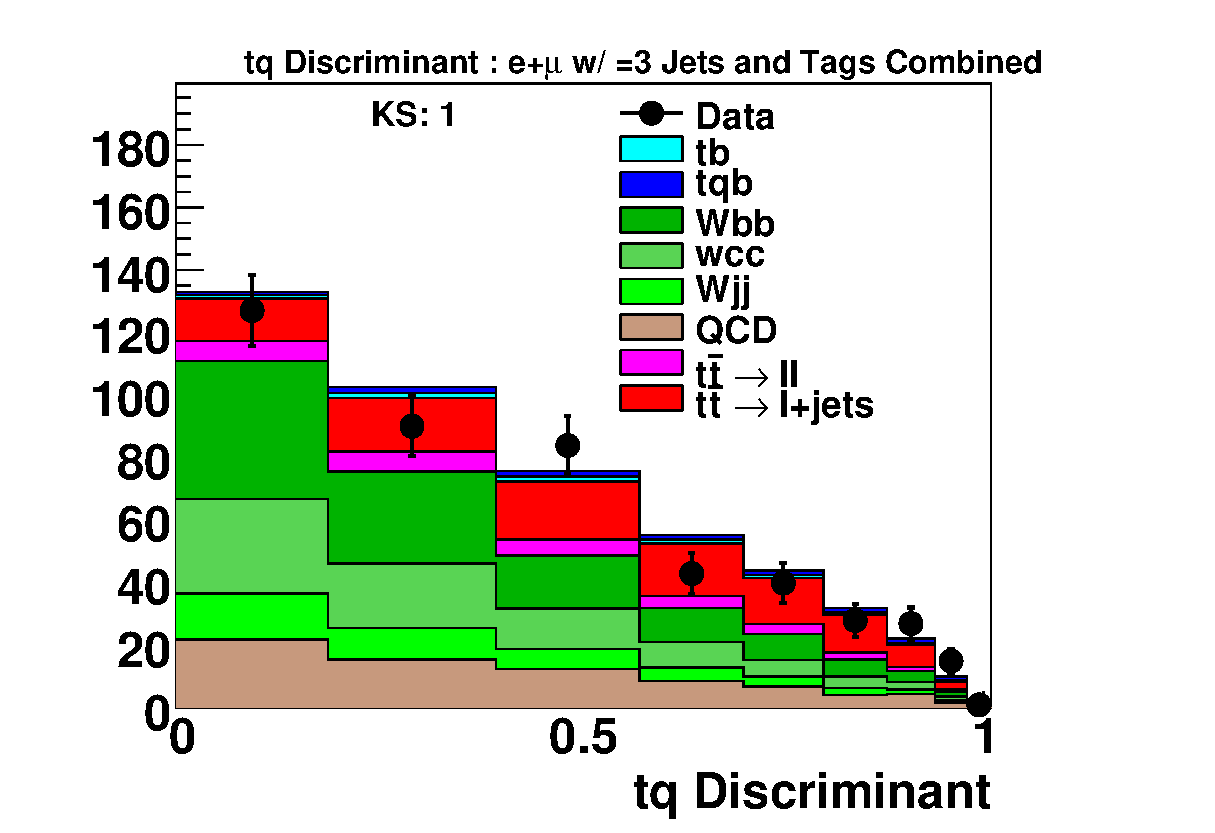
\includegraphics[width=0.36\textwidth]
{figures/output/3jet/All_tq_Discriminant.eps}
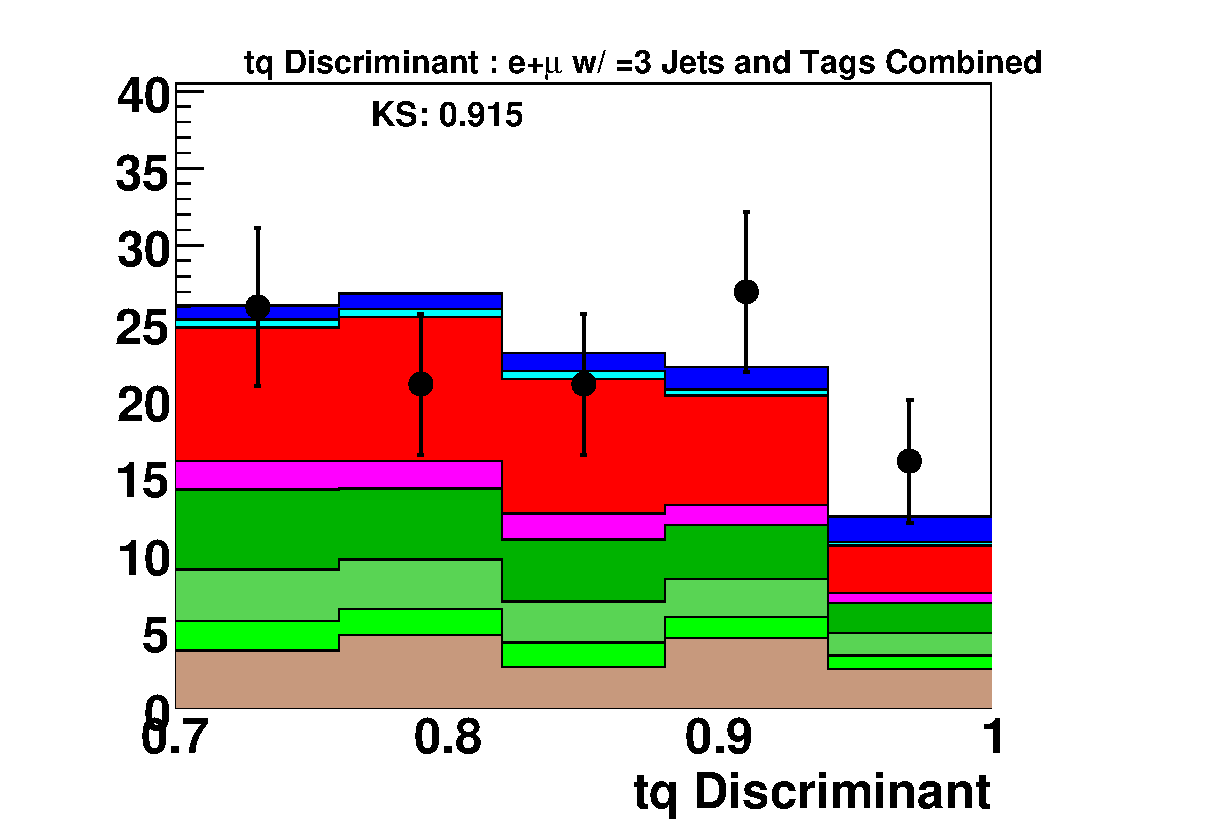
\includegraphics[width=0.36\textwidth]
{figures/output/3jet/All_tq_Discriminant_Zoom.eps}
\vspace{-0.1in}
\caption{Discriminant plots for the e+$\mu$ channel with three jets
and $\geq$~1 $b$~tag. Upper row: $tb$ discriminant; lower row: $tq$
discriminant. Left column: full output range; right column: close-up
of the high end of the distributions.}
\label{e21_3j}
\end{figure}

\clearpage

Figure~\ref{disc2d_data} shows the 2D discriminant distribution in
data for all analysis channels ($e$,$\mu$ / 1,2 tags), separately for
two-jet and three-jet events. This is the typ of distribution we use
for the single top quark cross section measurement, but we actually
use each different analysis channel separately.

\begin{figure}[!h!tbp]
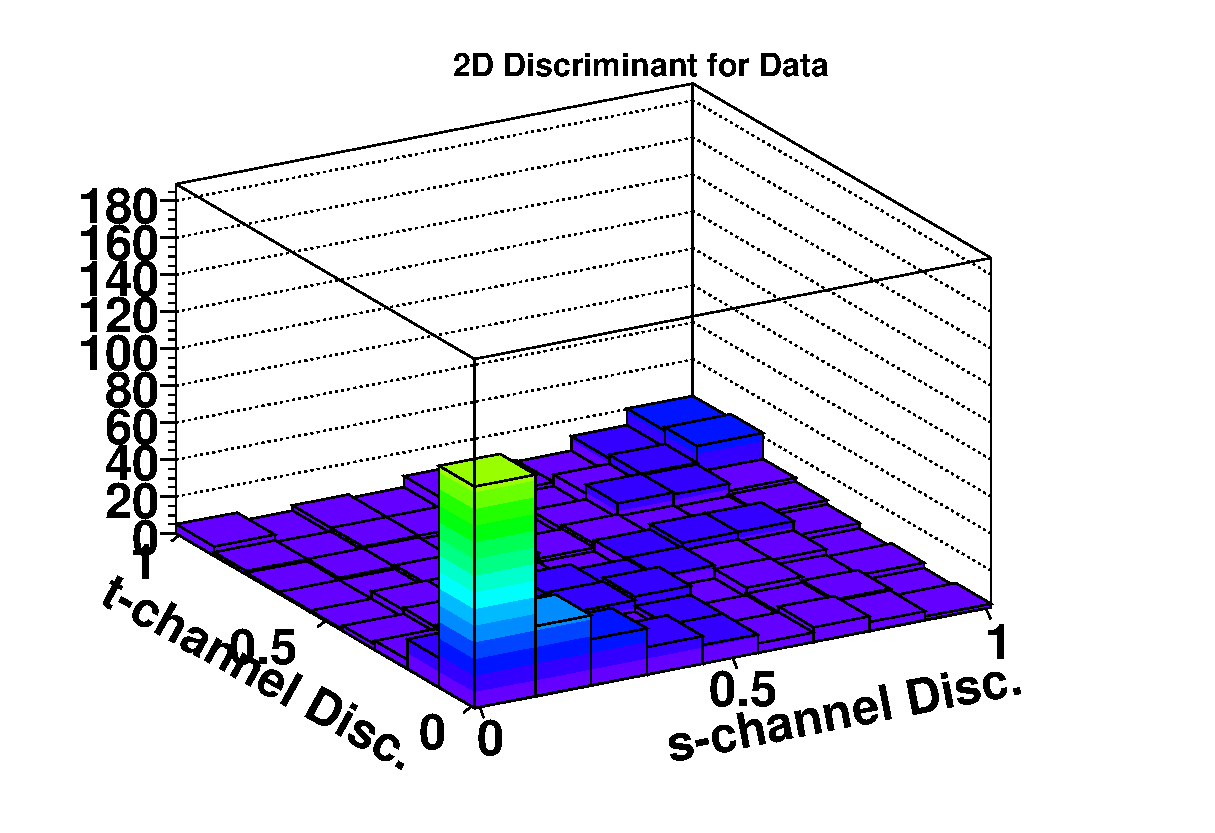
\includegraphics[width=0.45\textwidth]
{figures/performance/2D-Discriminant_data_2jet.eps}
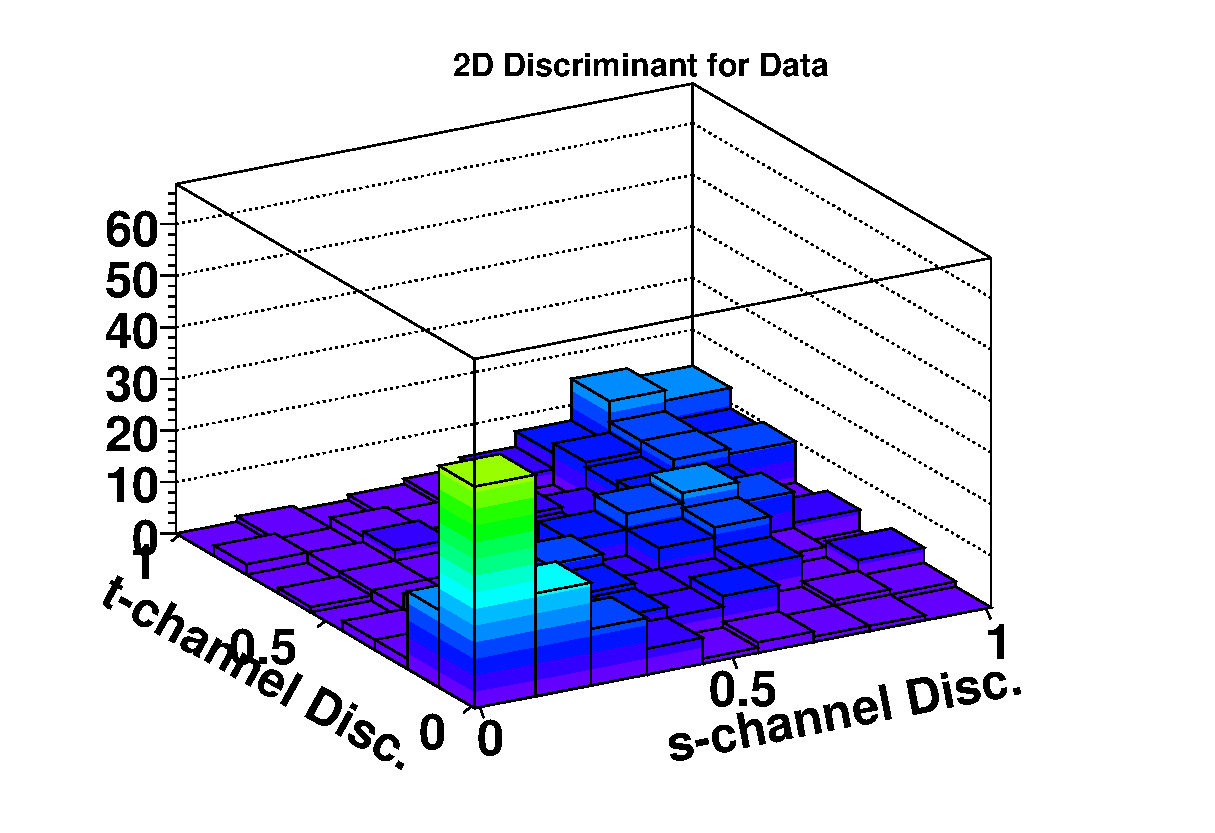
\includegraphics[width=0.45\textwidth]
{figures/performance/2D-Discriminant_data_3jet.eps}
\vspace{-0.1in}
\caption[disc2d_data]{2D discriminant distribution in data
($e$,$\mu$ / 1,2 tags combined) for two-jet (left) and three-jet
(right) events.}
\label{disc2d_data}
\end{figure}

\subsection{Measured Cross Section}

Figure~\ref{meas-post-1d} shows the observed $tb$+$tqb$ posterior
without and with systematic uncertainties for all channels combined.

\begin{figure}[!h!tbp]
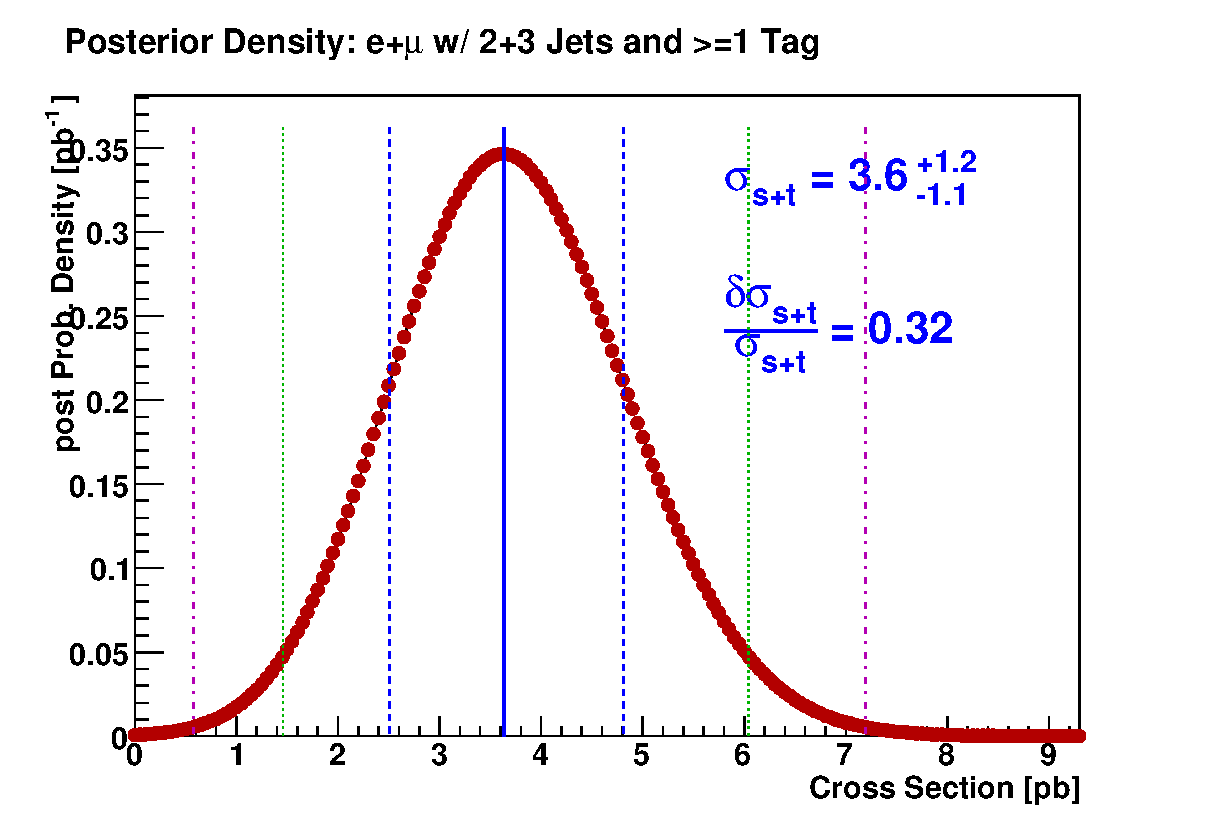
\includegraphics[width=0.36\textwidth]{figures/posterior/nosys/limit_TBTQ_LeptonsCombined_JetsCombined_TagsCombined.eps}
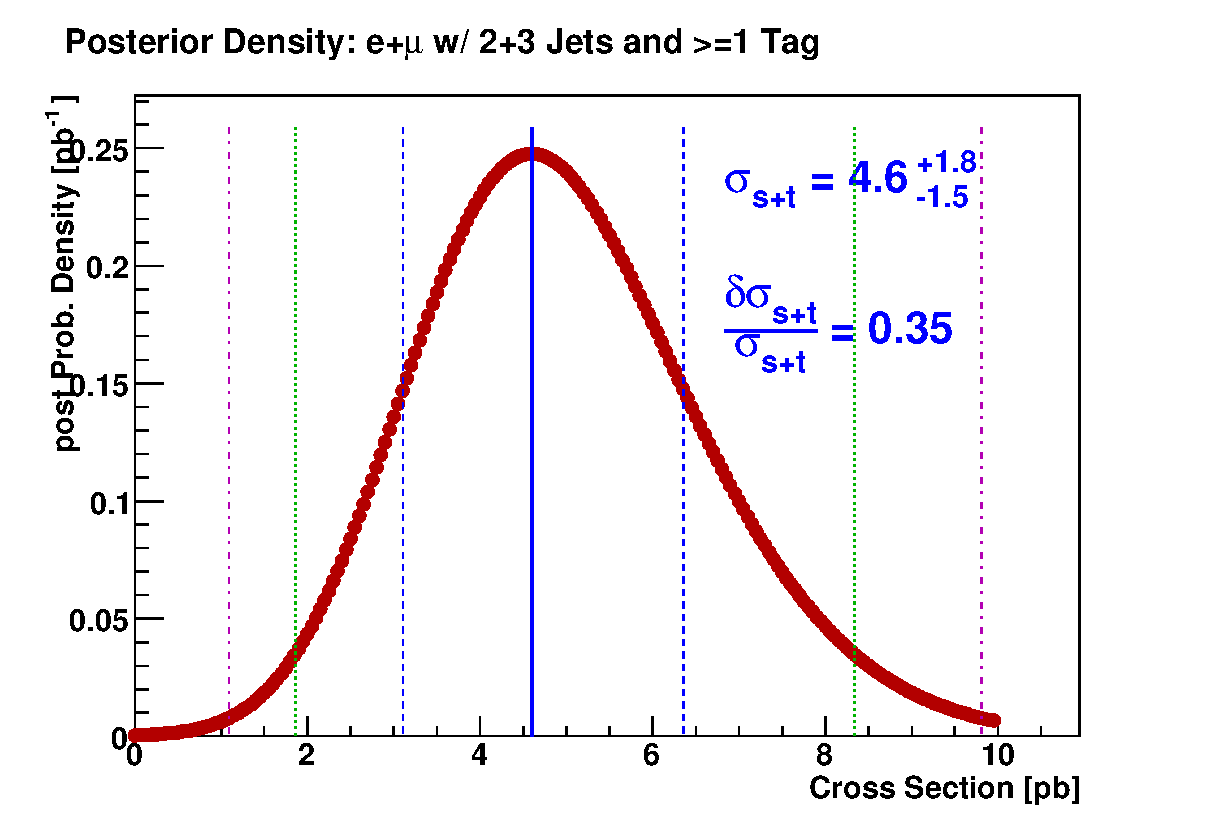
\includegraphics[width=0.36\textwidth]{figures/posterior/sys/limit_TBTQ_LeptonsCombined_JetsCombined_TagsCombined.eps}
\vspace{-0.1in}
\caption[measpost1d]{Measured 1D posterior plots for the combined
$e$+$\mu$ $\geq$~1 $b$-tag channel with statistical uncertainties only
(left plot) and with systematic uncertainties as well (right plot).}
\label{meas-post-1d}
\end{figure}

Table~\ref{tab:measxsecs} shows the measured cross sections from
various combinations of analysis channels.  The averaged relative
uncertainties on the measured cross sections are shown in
Table~\ref{meas-errors}.

\begin{table}[!h!tbp]
\begin{center}
\begin{minipage}{5in}
\begin{ruledtabular}
\begin{tabular}{l|cc|cc|cc|c}
  \multicolumn{8}{c}{\hspace{0.5in}\underline{Measured $tb$+$tqb$ Cross Section}}\vspace{0.1in}\\
& \multicolumn{2}{c|}{1,2tags + 2,3jets}& \multicolumn{2}{c|}{$e$,$\mu$ + 2,3jets}
& \multicolumn{2}{c|}{$e$,$\mu$ + 1,2tags}& All \\
                 &  $e$-chan & $\mu$-chan& 1 tag & 2 tags& 2 jets& 3 jets&channels\\
\hline
Statistics only  &  $3.0^{+1.5}_{-1.4}$  & $4.5^{+1.8}_{-1.7}$ & $2.8^{+1.2}_{-1.2}$ & $7.9^{+3.3}_{-3.0}$ & $3.5^{+1.4}_{-1.3}$ & $3.9^{+2.3}_{-2.2}$ & $3.6^{+1.2}_{-1.1}$     \\
With systematics &  $3.1^{+2.2}_{-1.8}$  & $7.4^{+3.0}_{-2.5}$ & $4.5^{+2.0}_{-1.7}$ & $6.8^{+4.7}_{-3.8}$ & $4.7^{+2.0}_{-1.7}$ & $4.9^{+3.7}_{-3.1}$ & $\mathbf{4.6^{+1.8}_{-1.5}}$     \\
\end{tabular}
\end{ruledtabular}
\vspace{-0.1in}
\caption[measxsecs]{Measured $tb$+$tqb$ cross sections, without and
with systematic uncertainties, for many combinations of the analysis
channels. The final result of this analysis is shown in the lower
right hand corner in bold type.}
\label{tab:measxsecs}
\end{minipage}
\end{center}
\end{table}

\begin{table}[!h!tbp]
\begin{center}
\begin{minipage}{5in}
\begin{ruledtabular}
\begin{tabular}{l|cc|cc|cc|c}
  \multicolumn{8}{c}{\hspace{0.5in}\underline{Relative Uncertainties on the Measured $tb$+$tqb$ Cross Section}}\vspace{0.1in}\\
& \multicolumn{2}{c|}{1,2tags + 2,3jets}& \multicolumn{2}{c|}{$e$,$\mu$ + 2,3jets}
& \multicolumn{2}{c|}{$e$,$\mu$ + 1,2tags}& All \\
                 &  $e$-chan & $\mu$-chan& 1 tag & 2 tags& 2 jets& 3 jets&channels\\
\hline
Statistics only  &  $50\%$  & $39\%$ & $44\%$ & $40\%$ &  $37\%$  & $57\%$ & $32\%$     \\
With systematics &  $64\%$  & $38\%$ & $41\%$ & $62\%$ &  $39\%$  & $70\%$ & $\mathbf{35\%}$     \\
\end{tabular}
\end{ruledtabular}
\vspace{-0.1in}
\caption[meas-errors]{Relative uncertainties on the measured
$tb$+$tqb$ cross section, without and with systematic uncertainties,
for many combinations of the analysis channels. The best value from
all channels combined, with systematics, is shown in bold type.}
\label{meas-errors}
\end{minipage}
\end{center}
\end{table}

The combined result with full systematics is
$$
\sigma\left({\ppbar}{\rargap}tb+tqb+X\right)
= 4.6 ^{+1.8}_{-1.5}~{\rm pb}.
$$

%\begin{figure}[!h!tbp]
%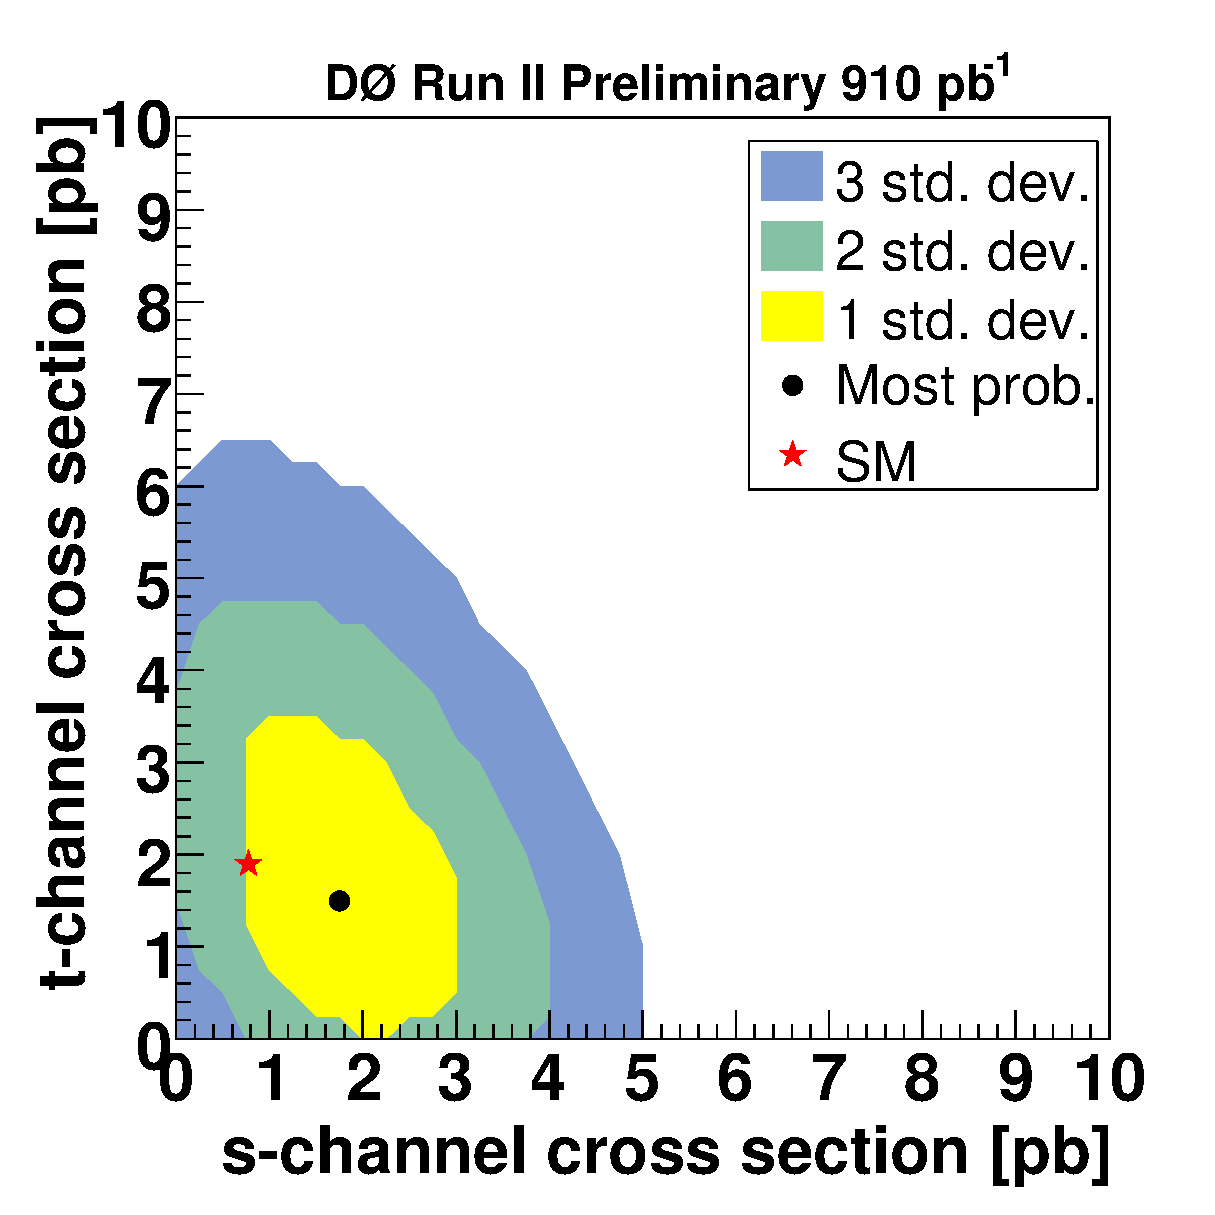
\includegraphics[width=0.35\textwidth]{figures/posterior/nosys/2D-Posterior_LeptonsCombined_2Jet_TagsCombined_limit.eps}
%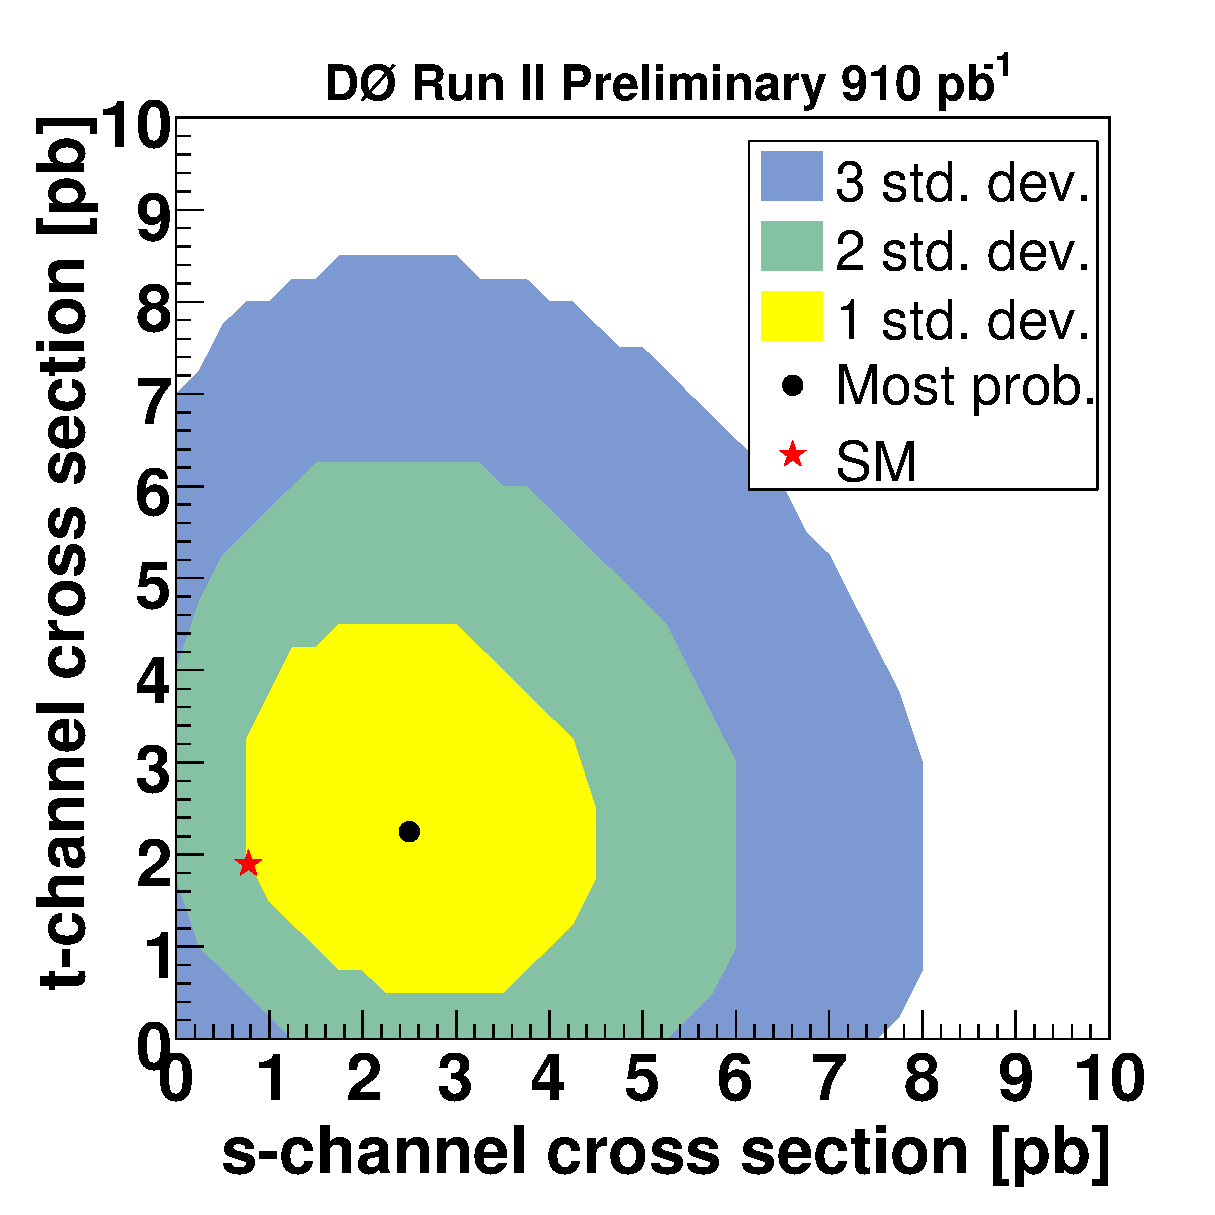
\includegraphics[width=0.35\textwidth]{figures/posterior/sys/2D-Posterior_LeptonsCombined_2Jet_TagsCombined_limit.eps}
%\vspace{-0.1in}
%\caption[measpost2d]{Measured 2D posterior plots for the combined
%$e$+$\mu$ $\geq$~1 $b$-tag channel with statistical uncertainties only
%(left plot) and with systematic uncertainties as well (right plot).}
%\label{meas-post-2d}
%\end{figure}

\noindent A breakdown of the uncertainties on the $tb$+$tqb$ cross
section measurement is given in Table~\ref{tab:syst}. The systematic
uncertainties were calculated using an ensemble containing 200
datasets generated with an input single top cross section of
4.7~pb. The cross section of each dataset was measured and the average
posterior width (average of upper and lower 1$\sigma$ uncertainties)
was calculated over all datasets for each source of systematic
uncertainty independently. The systematic uncertainty for each source
was estimated by subtracting in quadrature from the average posterior
width obtained with a particular source of systematic, the average
posterior width without systematic uncertainties. The total expected
systematic uncertainty is estimated by adding in quadrature all the
individual expected systematic uncertainties.  The statistical
uncertainty of the measurement is estimated by subtracting in
quadrature the total expected systematic uncertainty from the actual
total uncertainty.

\vspace{0.1in}
\begin{table}[!h!tbp]
\begin{center}
\begin{minipage}{3in}
\begin{ruledtabular}
\begin{tabular}{lr@{ pb~~}}
\multicolumn{2}{c}
{Contributions to the Cross Section Uncertainty}\vspace{0.05in}\\
\hline
\multicolumn{2}{l}{Systematics components} \\
~~Luminosity               & 0.69	\\ 
~~{\ttbar} cross section   & 0.74	\\ 
~~Matrix method            & 0.84	\\
~~Trigger                  & 0.48	\\ 
~~Primary vertex           & 0.31	\\
~~Lepton ID                & 0.50	\\
~~Jet ID                   & 0.18	\\
~~Jet fragmentation        & 0.63	\\
~~Jet energy scale         & 0.57	\\
~~Tag-rate functions       & 0.60	\\
\hline                     
Combined systematics       & +1.34~~$-1.02$ \\
Statistics                 & +1.19~~$-1.13$ \\
\hline
Total uncertainty          & +1.79~~$-1.50$ \\
\end{tabular}
\end{ruledtabular}
\vspace{-0.1in}
\caption[syst]{Contribution of each systematic uncertainty to the
total systematic uncertainty on the $tb$+$tqb$ cross section.}
\label{tab:syst}
\end{minipage}
\end{center}
\end{table}


Figure~\ref{xsec-summary} shows the cross sections measured for
combined $tb$+$tqb$ production in each independent analysis channel,
and the combined result, taken from the 1-d posterior density
distribution measurements.

\begin{figure}[!h!tbp]
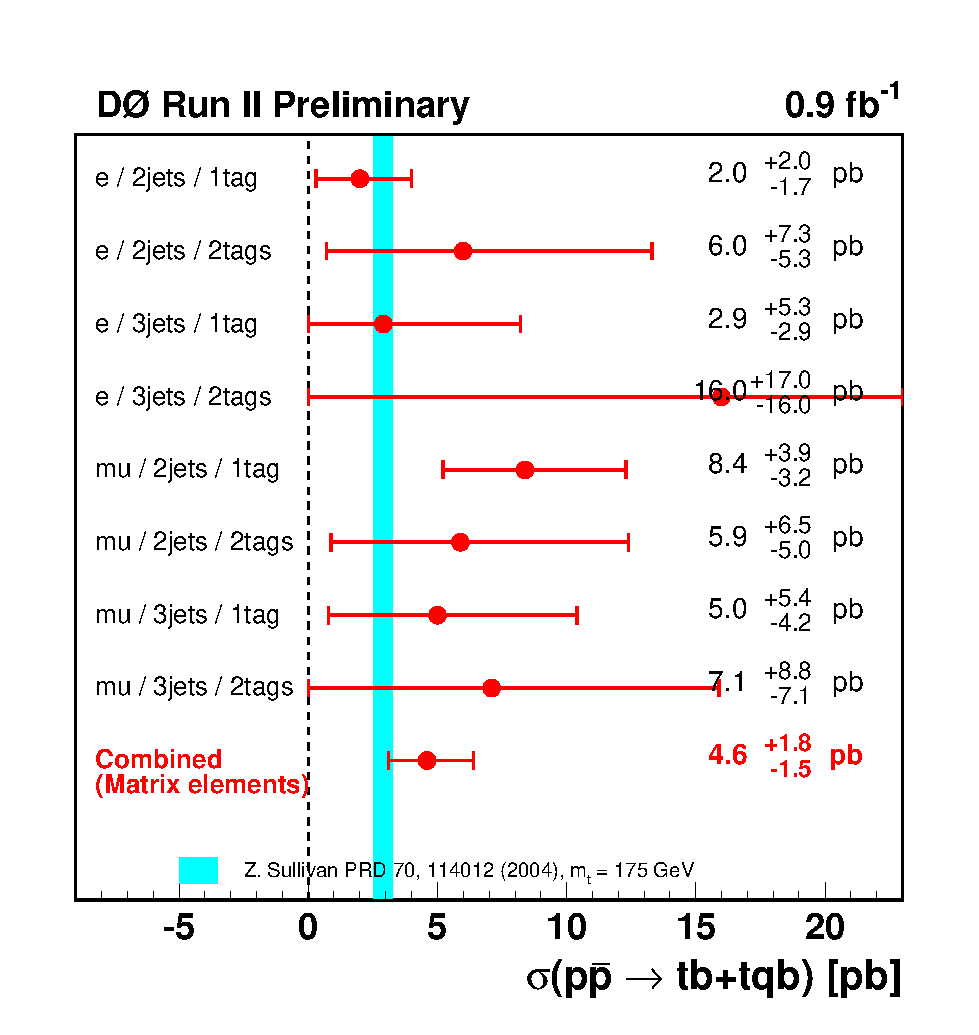
\includegraphics[width=0.55\textwidth]
{figures/sintop_xsec_summary.eps}
\begin{minipage}{4in}
\caption[xsecsumm]{Summary plot of the measured single top quark cross
sections showing the individual measurements and their combination.}
\label{xsec-summary}
\end{minipage}
\end{figure}


\section{Signal Significance}

We calculate the probability that the background alone could fluctuate
up to or above the measured cross section. This is known as the
p-value, see Appendix~10 in
Ref.~\cite{general-note}. Figure~\ref{pValue} shows the distribution
of cross sections for the zero-signal ensemble with full systematics
included. From this distribution, we calculate a p-value of 0.22\%,
which corresponds to a 2.9$\sigma$ fluctuation from zero.

\begin{figure}[!h!tbp]
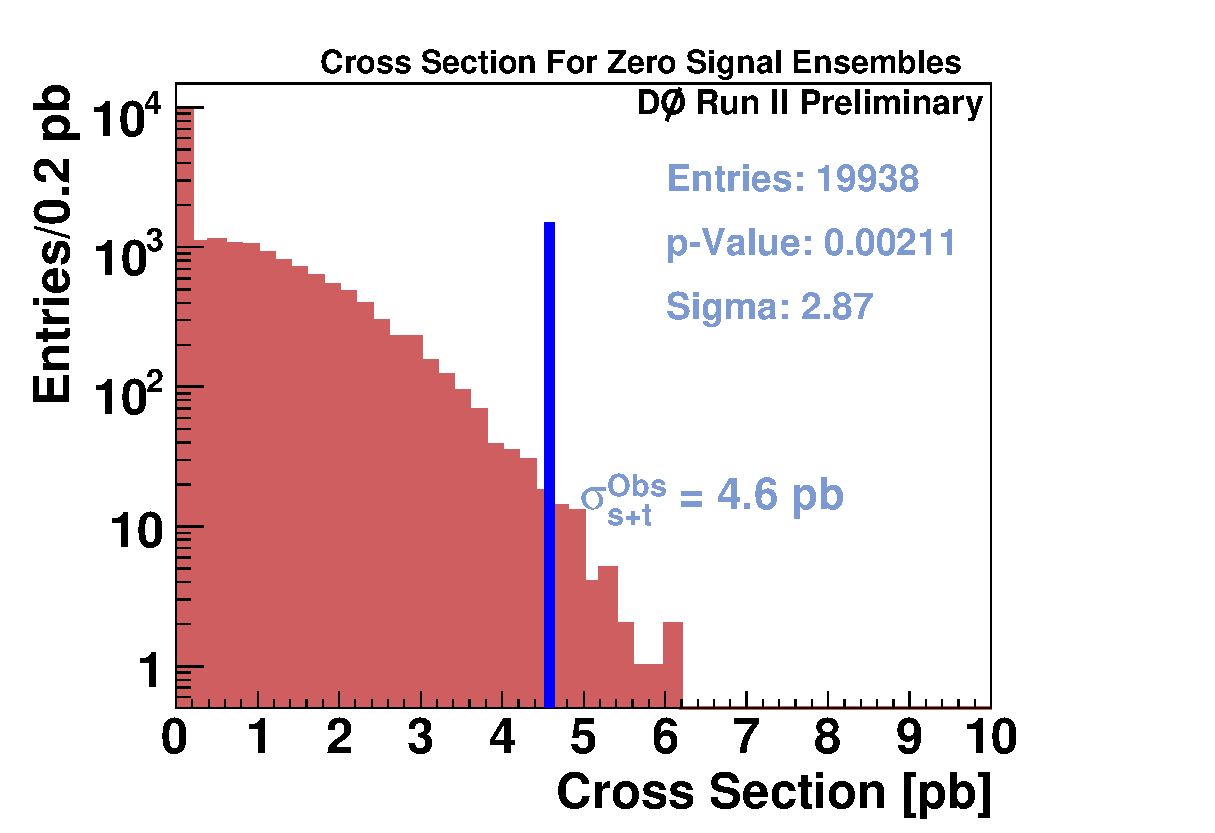
\includegraphics[width=0.55\textwidth]
{figures/ensembles/EnsemblesZero.eps}
\begin{minipage}{4in}
\caption[pValue]{Distribution of cross sections from a zero-signal
ensemble with full systematics included.}
\label{pValue}
\end{minipage}
\end{figure}

\clearpage

\section{Event Characteristics}
\label{sec:eventcharacteristics}

After the matrix element discriminant has been calculated, it is
possible to place a cut on this value to select events in data and
Monte Carlo to see if they are consistent with single top quark
production. For this section, an event is considered very single top
quark like if both the s-channel and t-channel discriminants are
greater than 0.7. Similarly, an event is considered background like if
both discriminants are less than 0.4. Figure~\ref{top-mass} shows the
invariant mass of the lepton, neutrino, and tagged jet before and
after the discriminant cut, and Fig.~\ref{q-eta} shows the
lepton-charge times pseudorapidity of the untagged jet.

\begin{figure}[!h!tbp]
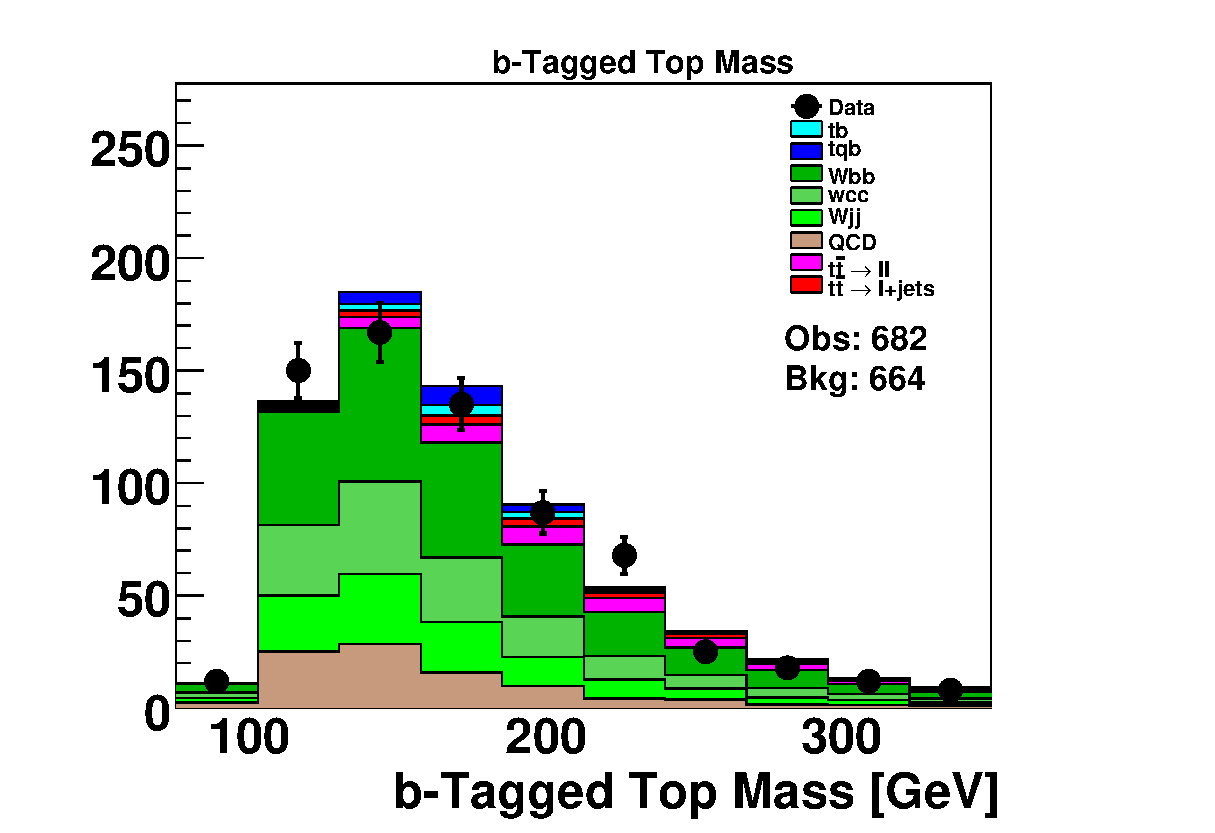
\includegraphics[width=0.32\textwidth]
{figures/topovars/BTaggedTopMass_0.eps}
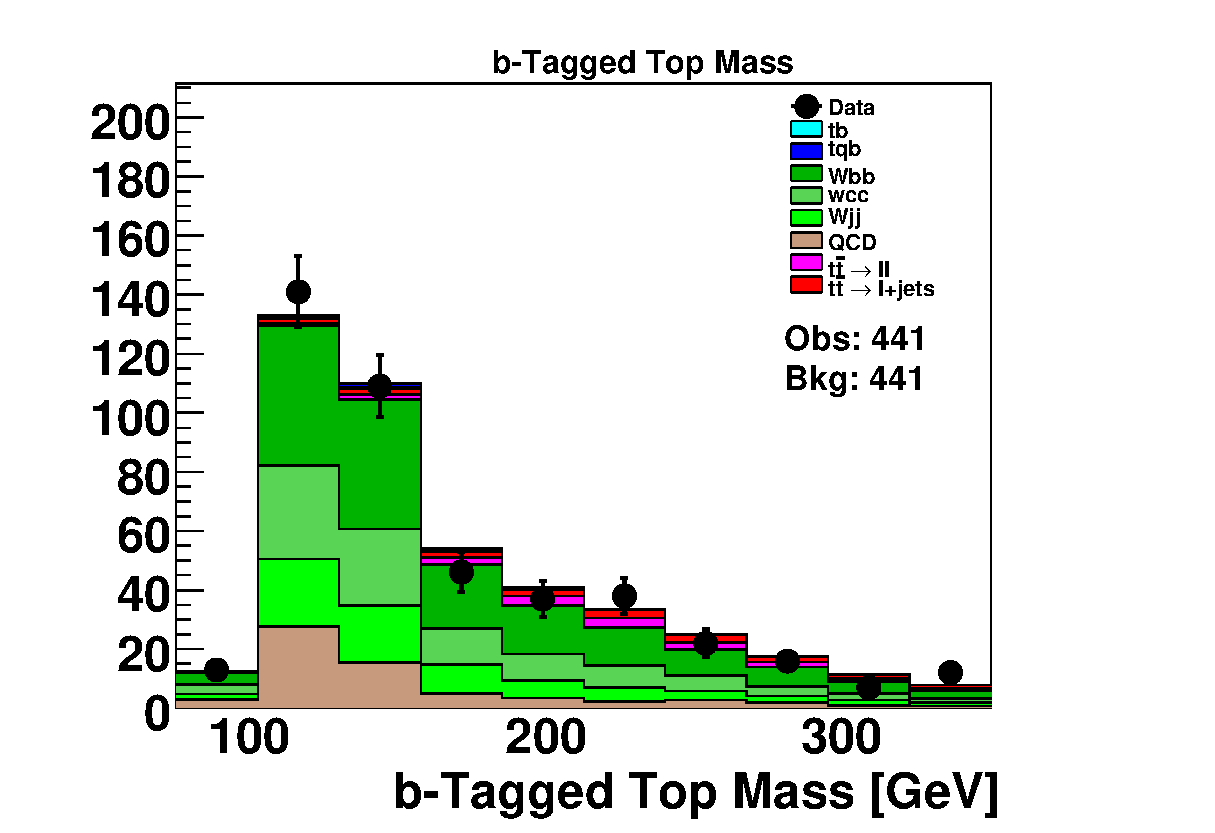
\includegraphics[width=0.32\textwidth]
{figures/topovars/BTaggedTopMass_-0.4.eps}
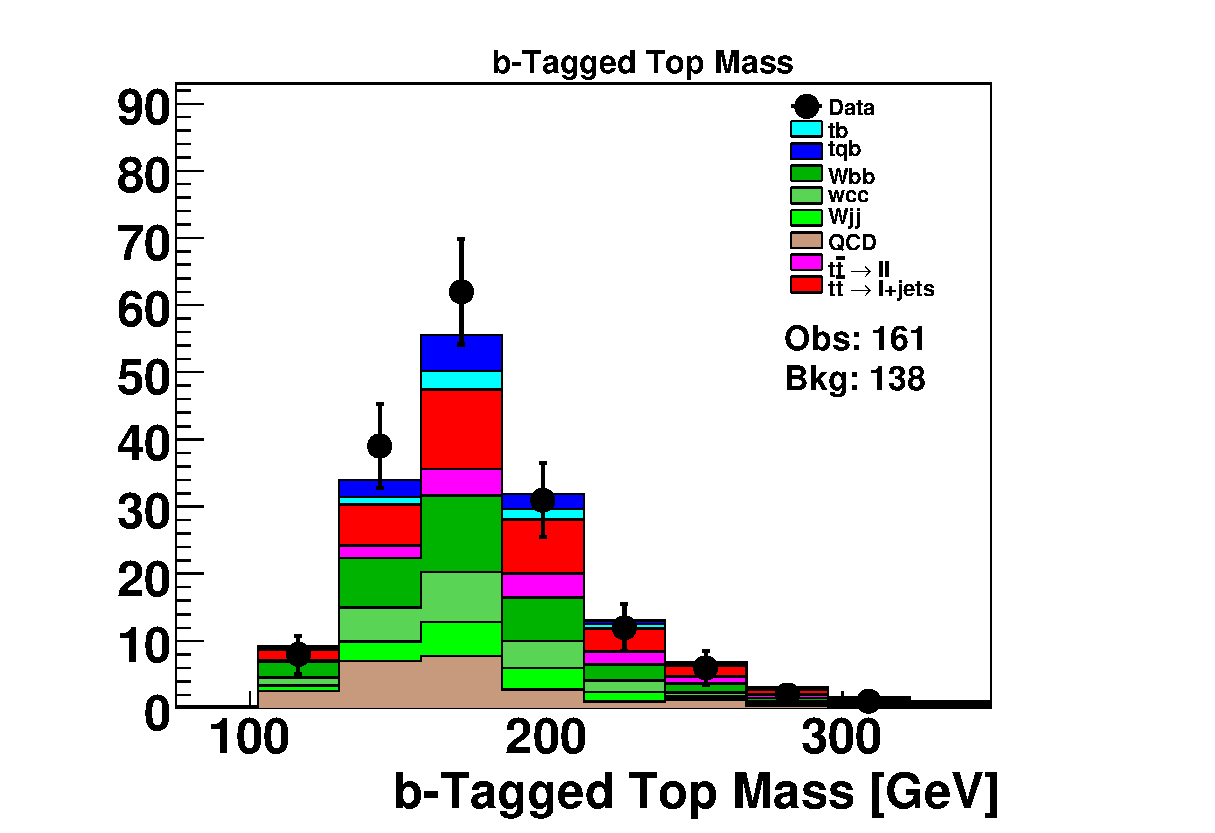
\includegraphics[width=0.32\textwidth]
{figures/topovars/BTaggedTopMass_0.7.eps}
\vspace{-0.1in}
\caption[topmass]{Invariant mass of the lepton, neutrino, and tagged
jet for all events (left plot), for events with $D < 0.4$ (middle
plot), and events with $D > 0.7$ (right plot).}
\label{top-mass}
\end{figure}

%\vspace{0.1in}
\begin{figure}[!h!tbp]
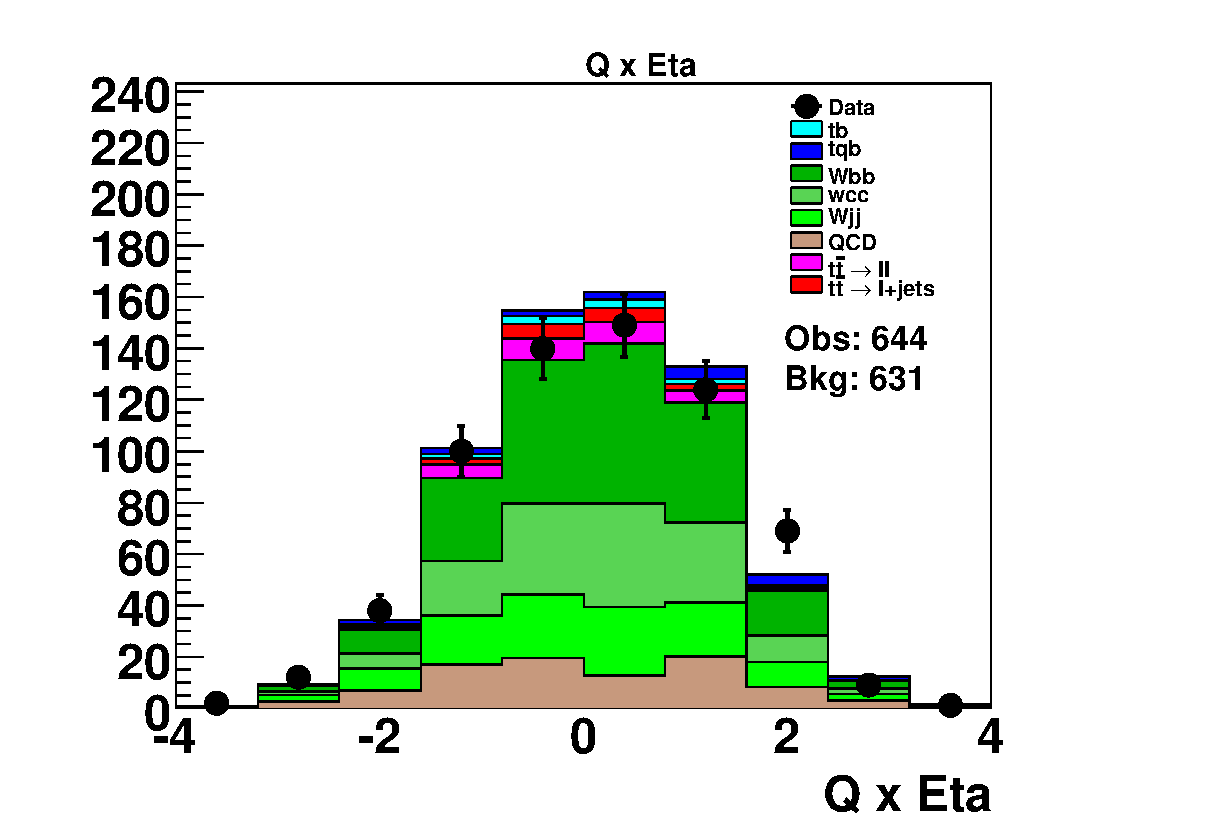
\includegraphics[width=0.32\textwidth]
{figures/topovars/QTimesEta_0.eps}
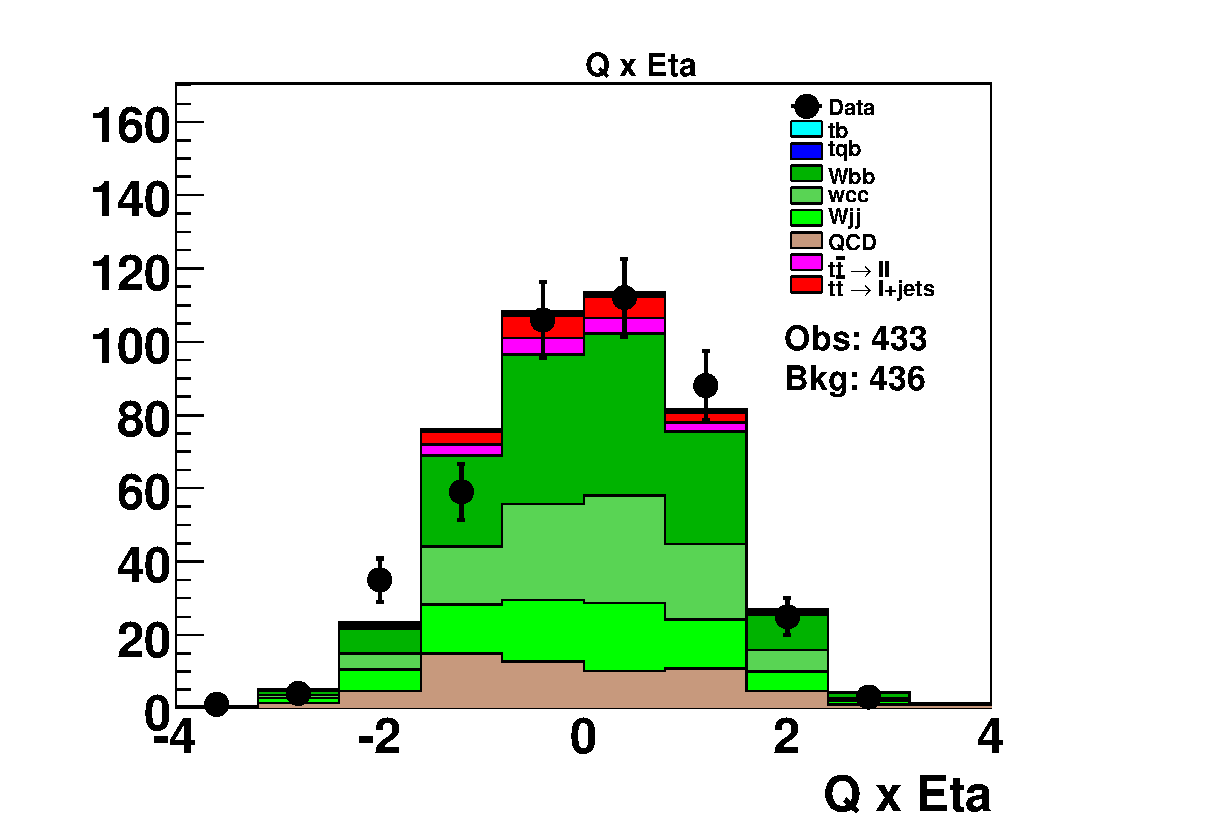
\includegraphics[width=0.32\textwidth]
{figures/topovars/QTimesEta_-0.4.eps}
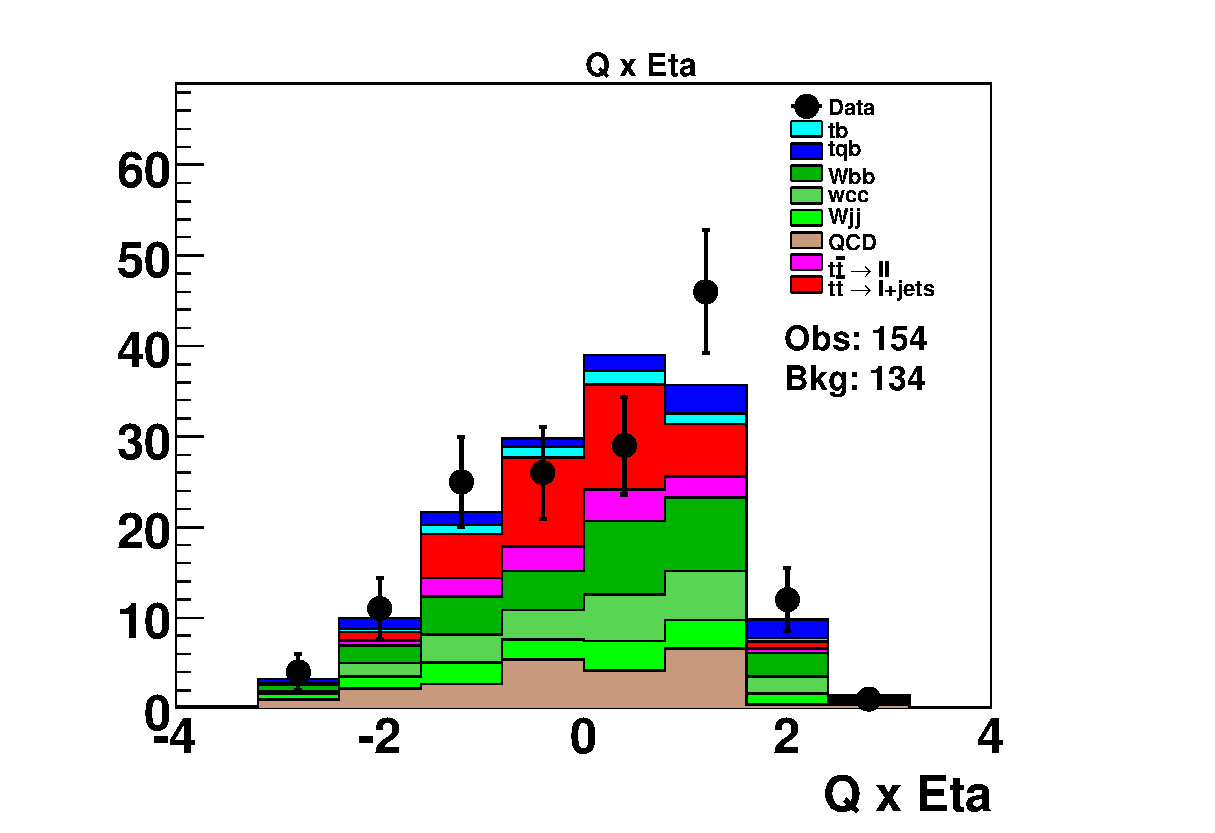
\includegraphics[width=0.32\textwidth]
{figures/topovars/QTimesEta_0.7.eps}
\vspace{-0.1in}
\caption[qeta]{Lepton charge times the pseudorapidity of the untagged
jet for all events (left plot), for events with $D < 0.4$ (middle
plot), and events with $D > 0.7$ (right plot). The number of observed
events is different from the $b$-tagged top mass plot because this
variable is only defined for events with at least one untagged jet.}
\label{q-eta}
\end{figure}
